\chapter{Experimentación y análisis}

\noindent Este capítulo separa las \textbf{verificaciones previas} de los \textbf{resultados experimentales}. La calidad y preparación de los datos se documentan en el Capítulo~5; las comprobaciones de reglas, integración y entorno confirman aquí que el sistema puede ejecutar el protocolo, pero no constituyen resultados de rendimiento. Sobre esa base se presentan dos bloques de resultados: \textbf{aprendizaje}, que incluye la señal supervisada y las políticas \acroref{MARL}{MARL}, y \textbf{económico}, que compara el comportamiento de una cartera conjunta con referencias homogéneas.

Esta distinción evita tres interpretaciones erróneas: que una prueba de funcionamiento demuestre rentabilidad, que una métrica interna de aprendizaje sea retorno de cartera o que la distribución de clases del conjunto constituya un resultado económico. El orden del capítulo sigue esa lógica: diseño y verificaciones previas, resultados de aprendizaje, resultados económicos y discusión.

\section{Diseño experimental}

El diseño experimental sigue el flujo de la arquitectura de las Figuras~\ref{fig:arquitectura-niveles} y~\ref{fig:arquitectura-estado-retroalimentacion}: adquisición y persistencia de datos, construcción del estado, señal supervisada, decisión conjunta de \textit{Scout}, \textit{Trader} y \textit{Portfolio}, y transición de la cartera simulada. La calidad del conjunto temporal se comprueba en el Capítulo~5 y las verificaciones de esta sección aseguran que cada componente produce entradas válidas para el siguiente. Solo después se entrenan los modelos y se calcula el resultado económico de la cartera.

La adquisición se realiza con un \emph{\glosref{scraping}{scraper}}, es decir, un programa que consulta fuentes web y transforma sus respuestas en datos estructurados, junto con persistencia de registros, sesiones y \emph{\glosref{cookie-sesion}{cookies de sesión}}, pequeños datos locales que permiten reutilizar una autenticación ya iniciada. Esta fase no se evalúa mediante rentabilidad, pero condiciona todos los experimentos posteriores: sin datos trazables, fechas de captura y sesiones reproducibles no se puede construir un histórico. Los bloqueos temporales, los cambios de interfaz y los límites de las plataformas obligan además a equilibrar cobertura, estabilidad de sesión y ritmo de captura.

\textbf{Señal supervisada.} A partir de los datos persistidos se construyen los conjuntos temporales y se entrenan modelos tabulares: regresión logística, \emph{random forest} e \emph{histogram gradient boosting} \cite{breiman2001random,friedman2001greedy}. Se contrastan con una referencia que predice la clase mayoritaria. Su salida es una probabilidad auxiliar incluida en el estado de los agentes; no constituye una orden de compra ni se interpreta como rentabilidad. Esta distinción es esencial en el conjunto Steam/\acroref{BUFF}{BUFF}, cuyo objetivo es estudiar una compraventa con precios normalizados, comisiones y horizonte temporal, no anticipar una variación aislada de precio.

\textbf{Entorno multiagente.} El simulador recibe el estado y la acción conjunta y comprueba compra, bloqueo, venta y trazabilidad. El entrenamiento usa \acroref{PPO}{PPO}, \emph{Proximal Policy Optimization}, que ajusta una política a partir de episodios simulados y limita el tamaño de cada actualización \cite{schulman2017ppo}. Se mantiene una política por rol: \textit{Scout}, \textit{Trader} y \textit{Portfolio}. La matriz compara configuraciones y semillas exclusivamente en validación; el conjunto de prueba se reserva para la evaluación independiente.

\begin{algorithm}[H]
\caption{Entrenamiento con PPO}
\label{alg:entrenamiento-ppo}
\begin{algorithmic}[1]
\Require Entorno paralelo, políticas \textit{Scout}, \textit{Trader} y \textit{Portfolio}, iteraciones y pasos
\Ensure Modelo guardado (\glosref{checkpoint}{punto de control}) y métricas de la ejecución
\State Inicializar una política \acroref{PPO}{PPO} por rol con observaciones vectoriales
\For{cada iteración de entrenamiento}
  \State Ejecutar episodios y registrar $(o_t^i,a_t^i,R_t,m_t^i)$
  \State Estimar ventajas $\widehat{A}_t$ a partir de las transiciones registradas
  \State Optimizar cada política con el objetivo recortado de \acroref{PPO}{PPO}
\EndFor
\State Evaluar el modelo guardado sin actualizar sus parámetros
\State Guardar efectivo, posiciones, operaciones y recompensa media
\end{algorithmic}
\end{algorithm}

El conjunto de prueba permaneció aislado durante la selección de la configuración. La evaluación independiente compara la política MARL seleccionada mediante validación con referencias homogéneas: mantener efectivo, comprar cuando el margen neto observado es positivo y una política PPO centralizada sujeta a las mismas restricciones. La comparación comunica el retorno de cartera, el beneficio neto, las operaciones cerradas, las posiciones abiertas y los rechazos por restricciones como media e intervalo entre semillas. La prueba se ejecutó una sola vez y no se ha reutilizado al ampliar la cuadrícula de validación.

\section{Verificaciones previas de la implementación}
\label{sec:validacion-tecnica}

Estas verificaciones no son un tercer eje de resultados. Su única finalidad es comprobar que las reglas económicas, la captura de datos, la persistencia, la inferencia supervisada, el simulador de cartera y el entorno multiagente producen salidas coherentes antes de interpretar el aprendizaje o el retorno. Un resultado numérico puede parecer válido aunque se haya calculado sobre datos mal normalizados, fechas desplazadas, comisiones incorrectas o acciones imposibles dentro del simulador.

La validación técnica se organiza en tres capas, alineadas con la arquitectura. La primera comprueba reglas aisladas del dominio y de la cartera: conversión de moneda, comisiones, bloqueo temporal, límites y etiquetas. La segunda comprueba el flujo de datos entre captura, normalización, persistencia, construcción de conjuntos y carga de modelos. La tercera comprueba la transición del entorno multiagente: episodios de compra, mantenimiento, venta y rechazo que registran observaciones, acciones, recompensas y estado de cartera. La Tabla~\ref{tab:cobertura-pruebas} relaciona cada bloque con el riesgo que controla.

\textbf{Reglas económicas.} Antes de los experimentos se han convertido las reglas del procedimiento manual en funciones comprobables: conversión entre \acroref{EUR}{EUR} y \acroref{CNY}{CNY}, factores de comisión, cálculo de beneficio neto, rentabilidad porcentual, fecha de desbloqueo y capital bloqueado. Esta migración no demuestra rentabilidad por sí misma, pero garantiza que los experimentos posteriores usan las mismas reglas económicas y parámetros explícitos. Las pruebas unitarias reducen el riesgo de errores silenciosos y permiten repetir cada experimento con la misma configuración.

El conjunto de pruebas automatizadas combina tres tipos de comprobación ya descritos en el Capítulo~6: ejecución de casos con \glosref{pytest}{Pytest}, revisión estática con \glosref{ruff}{Ruff} y comprobación de tipos con \glosref{mypy}{Mypy}. En esta sección no se valoran por la herramienta empleada, sino por el riesgo que reducen. Las pruebas unitarias comprueban el comportamiento determinista del simulador, las reglas económicas del procedimiento manual, el \acroref{OCR}{OCR}, los conectores de mercado, los conjuntos supervisados, el conjunto de compraventa, el servicio de evaluación de oportunidades y los componentes \acroref{MARL}{MARL}. La prueba de integración de persistencia se mantiene separada porque necesita una base de datos disponible.

\begin{table}[h]
\centering
\begin{tabularx}{\textwidth}{>{\raggedright\arraybackslash}p{0.27\textwidth} >{\raggedright\arraybackslash}X}
\toprule
Bloque & Riesgo controlado \\
\midrule
Reglas y cartera & Cálculos económicos incorrectos o posiciones imposibles. \\
Datos y captura & Registros incompletos, mal normalizados o sin trazabilidad temporal. \\
Modelo supervisado & Variables incompatibles, modelos no cargables o inferencia incoherente. \\
Simulación \acroref{MARL}{MARL} & Acciones inválidas, recompensas mal asignadas o estado de cartera inconsistente. \\
Interfaz y operación & Comandos inseguros, estados poco claros o recomendaciones no revisables. \\
\bottomrule
\end{tabularx}
\caption{Cobertura de pruebas.}
\label{tab:cobertura-pruebas}
\end{table}

Las reglas económicas pertenecen a la primera capa; los conectores, la persistencia, los conjuntos, el OCR y la carga de modelos cubren la segunda; y los episodios MARL y la interfaz de consulta cubren la tercera. Estas comprobaciones validan que el sistema mide y registra de manera controlada; no demuestran por sí mismas que una estrategia sea mejor que otra.

\textbf{Resultados de las verificaciones.} La suite completa se ejecutó el 14 de agosto de 2026: 279 pruebas unitarias y 3 de integración, 282 en total, superadas en 24,94 segundos. Las pruebas de integración registran una instantánea de mercado, verifican una actualización de cotización y guardan una señal vinculada a un artículo dentro de una transacción que se revierte al terminar. Por tanto, no incorporan datos de prueba al histórico experimental.

\begin{table}[htbp]
\centering
\begin{tabularx}{\textwidth}{>{\raggedright\arraybackslash}p{0.25\textwidth} r >{\raggedright\arraybackslash}X}
\toprule
Bloque & Pruebas & Alcance \\
\midrule
Unitarias & 279 & Economía, OCR, conectores, captura web, conjuntos, simulador, MARL y panel web. \\
Integración & 3 & Instantáneas, actualización de precios y señales en PostgreSQL. \\
Suite completa & 282 & Todas superadas en 24,94 segundos. \\
\bottomrule
\end{tabularx}
\caption{Resultados de las pruebas automatizadas.}
\label{tab:pruebas-recuperadas}
\end{table}

La validación de OCR es funcional y no comunica una tasa de exactitud no medida. El analizador construye observaciones con artículo, calidad, plataforma, precio, moneda y volumen; rechaza una confianza de 0,2 cuando el mínimo es 0,5; y completa el recorrido de carga, preprocesado y reconocimiento, con confianza 0,91 en el caso preparado. El OCR se considera, por tanto, un conector validado, no un reconocedor cuantificado sobre un corpus de capturas.

También se comprobó el entorno multiagente antes de entrenar. El caso controlado compra una unidad por 10,00~EUR el 1 de enero de 2026, mantiene la venta bloqueada hasta el 9 de enero y, al venderla por 14,00~EUR brutos en Steam, registra 12,18~EUR netos: la cartera pasa de 100,00 a 102,18~EUR. Un recorrido determinista de 95 observaciones verifica además compras, espera, ventas, límites y reutilización de efectivo; una ejecución mínima de PPO completa una iteración y 64 pasos. Son verificaciones de transición y trazabilidad; no se utilizan en la comparación económica entre políticas.

\paragraph{Criterios de evaluación.}
\label{sec:metricas-experimentacion}

La calidad de datos y las verificaciones técnicas anteriores son requisitos de validez. Los resultados experimentales se evalúan únicamente en dos planos: aprendizaje y comportamiento económico. Ninguno sustituye al otro: una señal puede ser estadísticamente correcta y no superar costes de transacción, y una política puede modificar sus acciones sin mejorar la cartera.

\begin{itemize}
  \item \textbf{Aprendizaje.} Reúne los dos modelos que intervienen en la decisión. La señal supervisada se evalúa con precisión, \textbf{\glosref{exhaustividad}{exhaustividad}} o \emph{recall}, \acroref{F1}{F1}, \acroref{ROC-AUC}{ROC-AUC}, \acroref{PR-AUC}{PR-AUC}, \textbf{\emph{\glosref{brier-score}{Brier score}}} y calibración de probabilidades \cite{powers2011evaluation,saito2015pr,niculescu2005predicting,guo2017calibration}; así se comprueba si la probabilidad incorporada al estado aporta información histórica. Para MARL se registran la recompensa común y las recompensas por rol, la entropía y las probabilidades de acción de \textit{Scout}, \textit{Trader} y \textit{Portfolio}. La pérdida de valor del crítico, la fracción de recorte y la divergencia KL aproximada permiten detectar actualizaciones inestables. Estas métricas muestran cambios internos de las políticas y no se confunden con el retorno económico de cartera.

  \item \textbf{Aspectos económicos.} Miden el efecto conjunto de las decisiones MARL y de las referencias sobre una única cartera. Se comunican beneficio neto, retorno porcentual, efectivo y valor final de cartera, capital bloqueado, operaciones cerradas, posiciones abiertas y rechazos por restricciones. El \textbf{\emph{\glosref{drawdown}{drawdown}}} se registra como máxima caída de valor; si resulta nulo por las características del recorrido simulado, se comunica como una limitación y no como evidencia de ausencia de riesgo.
\end{itemize}

Por tanto, una conclusión de calidad predictiva o de aprendizaje MARL se formula en el primer plano, mientras que una conclusión de rentabilidad, uso de capital o riesgo de cartera se formula en el segundo.

\section{Resultados de aprendizaje}

Esta sección presenta exclusivamente resultados de los dos modelos que intervienen en la decisión: la señal supervisada y las políticas MARL. La composición, cobertura y distribución del conjunto utilizado se han comprobado previamente en la Sección~\ref{sec:calidad-conjunto-experimental}; esas comprobaciones son condiciones de validez de los experimentos, no resultados de aprendizaje ni de cartera.

\subsection{Exploraciones supervisadas}

\textbf{Exploración de dirección en Steam.} La fase supervisada conserva una exploración de dirección Steam con 47.467 filas de entrenamiento, 19.252 de validación y 18.412 de prueba. En este contexto, la etiqueta vale uno cuando el precio futuro de Steam supera el precio observado, y vale cero en el caso contrario. No representa una compraventa entre plataformas ni incorpora comisiones, por lo que no mide beneficio neto. Esta exploración sirve para comprobar que el flujo de variables, entrenamiento, calibración y selección por umbral funciona con una muestra de mayor tamaño, pero no se utiliza para aprobar compras. Los experimentos de compraventa BUFF--Steam se presentan a continuación y se apoyan en el procedimiento temporal descrito en la Sección~\ref{sec:calidad-conjunto-experimental}.

\begin{table}[h]
\centering
\begin{tabular}{c r r r}
\toprule
Umbral & Precisión & Exhaustividad & Señales \\
\midrule
0,50 & 0,716 & 0,116 & 1.293 \\
0,70 & 0,856 & 0,019 & 180 \\
0,80 & 0,947 & 0,011 & 95 \\
0,85 & 0,962 & 0,006 & 53 \\
0,90 & 1,000 & 0,003 & 22 \\
\bottomrule
\end{tabular}
\caption{Umbrales de dirección Steam.}
\label{tab:umbrales-direccion-steam}
\end{table}

El umbral 0,85 deja 53 señales de las 18.412 filas de prueba. Esto ilustra el intercambio entre precisión y cobertura: elevar el umbral selecciona menos casos y no convierte la probabilidad en una orden. La calibración se revisa porque una probabilidad solo es útil si representa de forma razonable la frecuencia observada \cite{niculescu2005predicting,guo2017calibration}. Estos resultados no se consideran definitivos ni equivalentes a rentabilidad. Sí indican que el flujo de entrenamiento, calibración, selección por umbral y evaluación temporal funciona antes de integrarse como señal auxiliar en el problema de compraventa.

\textbf{Exploraciones de compraventa BUFF--Steam.} La exploración utiliza el corte de marzo descrito como diagnóstico de calidad en la Sección~\ref{sec:calidad-conjunto-experimental}. Cada ejemplo representa la posibilidad de comprar un artículo en BUFF y venderlo en Steam tras un horizonte de ocho días. La etiqueta vale uno cuando, después de aplicar las comisiones configuradas, el retorno supera el 10\%. El precio de compra se toma de BUFF y el precio de venta de Steam se valora con el factor de venta de 0,87 empleado por el simulador.

El orden temporal se conserva en todas las fases. Para el corte de marzo se han usado 171 ejemplos de entrenamiento, 76 de validación y 95 de prueba. El entrenamiento termina el 20 de enero, la validación ocupa del 2 al 20 de febrero y la prueba comprende del 4 al 28 de marzo. Se eliminan ocho días antes de cada frontera para que el horizonte futuro de una observación no alcance el bloque siguiente. Ningún parámetro se modifica al consultar la prueba. Esta separación evita mezclar pasado y futuro, una precaución esencial cuando las observaciones tienen dependencia temporal \cite{bergmeir2018cv}.

\begin{figure}[htbp]
\centering
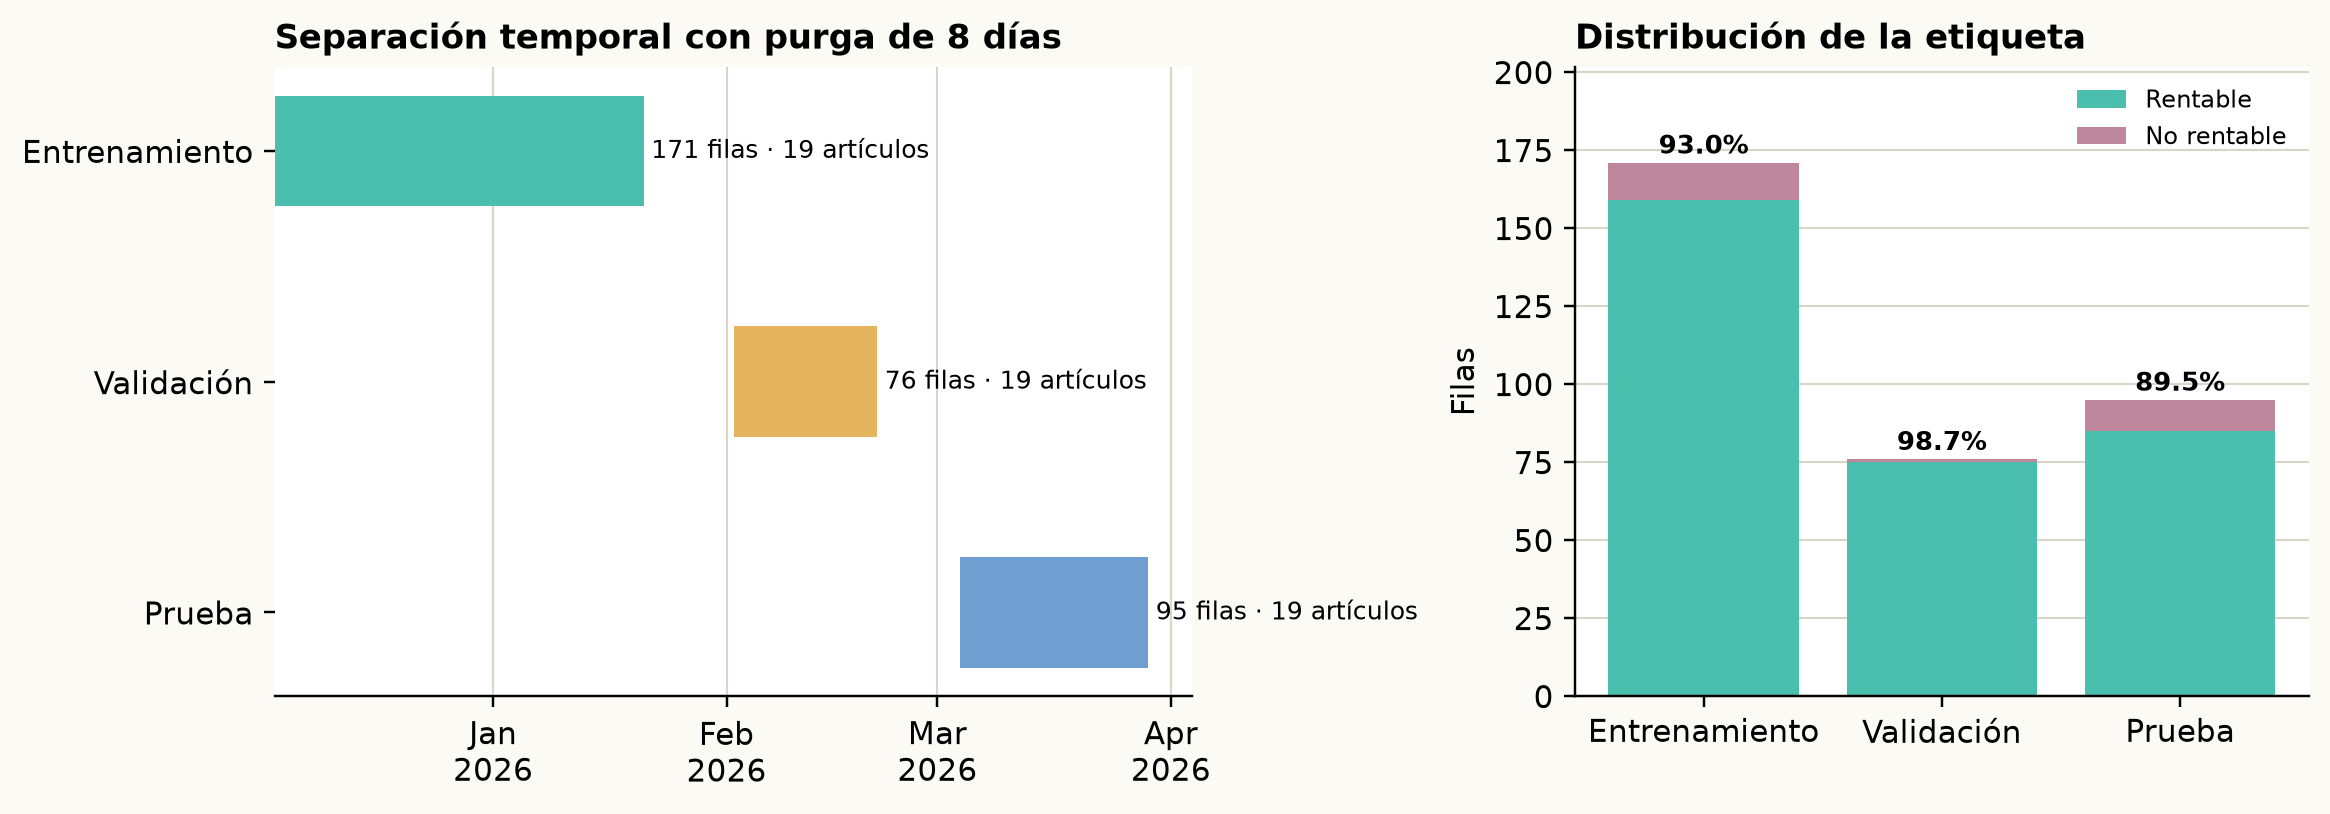
\includegraphics[width=\textwidth]{figures/experimentacion/03_cobertura_temporal.png}
\caption{Corte temporal de marzo.}
\label{fig:cobertura-marzo}
\end{figure}

La Figura~\ref{fig:cobertura-marzo} muestra una limitación que no se aprecia al mirar solo el número de filas. Los tres bloques contienen las mismas 19 representaciones de artículo y están dominados por la clase rentable. La separación temporal evita que se use información futura, pero no demuestra por sí sola que el modelo generalice a artículos que no ha visto durante el entrenamiento.

La selección compara las familias \emph{dummy}, regresión logística, \emph{random forest} e \emph{histogram gradient boosting}. El modelo \emph{dummy} se utiliza exclusivamente como referencia de frecuencia base y no tiene parámetros que explorar, por lo que no aparece en la Tabla~\ref{tab:configuraciones-marzo}. La configuración se elige en validación mediante precisión al umbral 0,85 con al menos tres señales. Después se calibra con sigmoide y se mide sobre el bloque de prueba. Además, se ejecuta una ablación de la regresión logística sin retardos, cambios, retornos ni medias móviles de uno, tres y siete días. Esta comparación responde a una pregunta concreta: si el histórico añade información o solamente complejidad. La precisión se presenta junto a la cobertura porque una clase mayoritaria puede hacer que el \acroref{ROC-AUC}{ROC-AUC} parezca más concluyente de lo que permite la muestra \cite{saito2015pr}.

La exploración no se ha limitado a escoger una familia. La Tabla~\ref{tab:configuraciones-marzo} recoge el espacio de búsqueda empleado. El conjunto de prueba ha quedado fuera de esta selección: sus valores se han consultado una vez después de fijar la configuración de validación.

\begin{table}[htbp]
\centering
\begin{tabularx}{\textwidth}{>{\raggedright\arraybackslash}p{0.25\textwidth} >{\raggedright\arraybackslash}X}
\toprule
Familia & Configuraciones exploradas \\
\midrule
Regresión logística & Regularización L2 con $C \in \{0{,}3, 1, 3\}$. \\
\emph{Random forest} & Profundidad 10 o 18, 160 árboles y cinco muestras por hoja. \\
HGB & Tasa de aprendizaje 0,05 o 0,10, 160 iteraciones y 31 hojas. \\
\bottomrule
\end{tabularx}
\caption{Configuraciones de marzo.}
\label{tab:configuraciones-marzo}
\end{table}

\begin{table}[htbp]
\centering
\begin{tabular}{l r r r r}
\toprule
Configuración & ROC-AUC & \emph{Brier} & Precisión @0,85 & Señales \\
\midrule
Logística con histórico & 0,641 & 0,075 & 0,929 & 85 \\
Logística sin histórico & 0,760 & 0,072 & 0,970 & 67 \\
\emph{Random forest} con histórico & 0,742 & 0,074 & 0,942 & 86 \\
HGB con histórico & 0,649 & 0,082 & 0,915 & 82 \\
\bottomrule
\end{tabular}
\caption{Comparativa de marzo.}
\label{tab:resultados-marzo}
\end{table}

\begin{figure}[H]
\centering
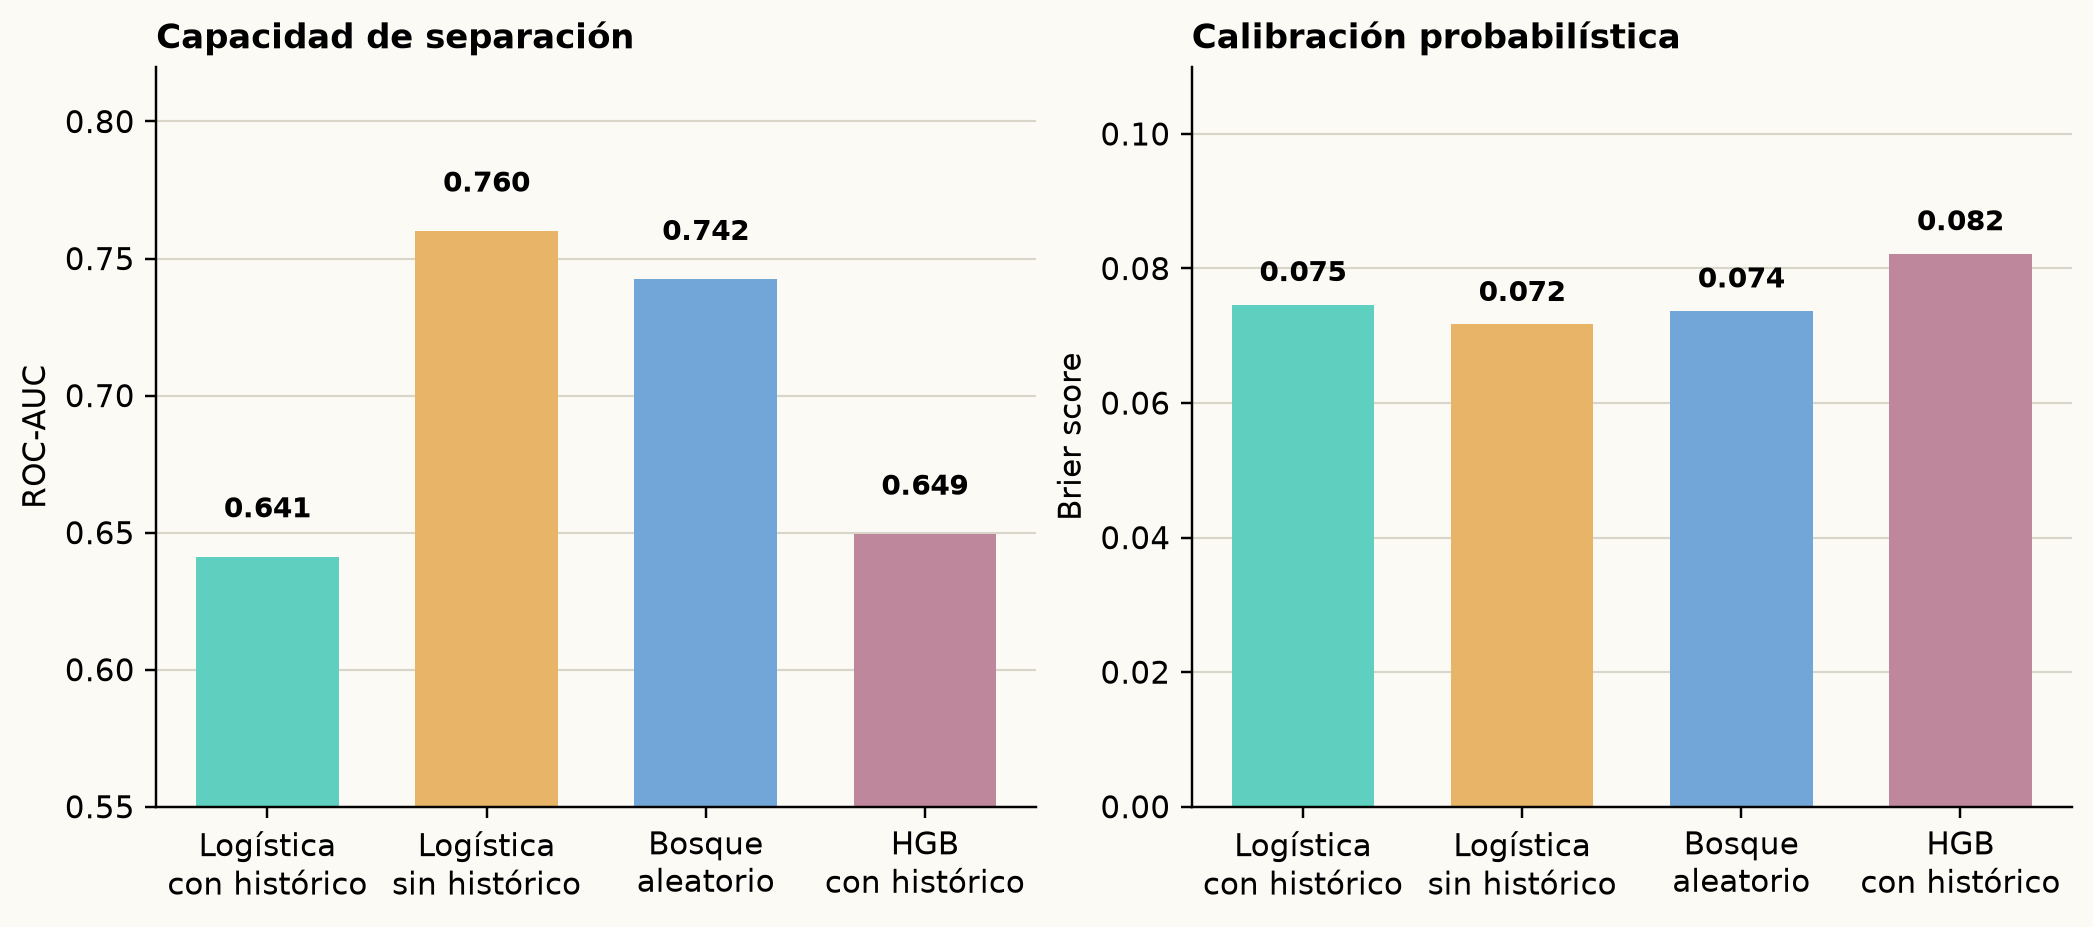
\includegraphics[width=\textwidth]{figures/experimentacion/01_modelos_marzo.png}
\caption{Modelos en marzo.}
\label{fig:modelos-marzo}
\end{figure}

La exploración inicial señala que la regresión logística sin características históricas puede separar mejor las dos clases que las alternativas probadas. También muestra que los retardos y medias móviles no deben darse por útiles sin contrastarlos. La siguiente ablación vuelve a medir esa decisión junto con la aumentación, usando particiones por fecha para que una fecha completa no se divida entre lados de un pliegue.

\textbf{Ablación de variables históricas y aumentación.} La segunda exploración usa una matriz $2 \times 2$ con regresión logística. Se mantienen los mismos cortes temporales de marzo, el umbral de selección 0,85, tres pliegues temporales y calibración sigmoide. Se comparan dos decisiones de diseño: conservar o retirar las variables históricas, formadas por retardos y medias móviles, y entrenar con o sin aumentación numérica. La aumentación se contrasta como hipótesis y no se presupone beneficiosa, ya que su efecto depende del dominio y del volumen de datos \cite{iwana2021augmentation}.

La aumentación se aplica únicamente al entrenamiento. Para cada variable numérica se genera una copia perturbada mediante

\[
x'_k=x_k+\varepsilon_k,
\qquad
\varepsilon_k \sim \mathcal{N}(0, 0{,}01 \cdot IQR(x_k)).
\]

En esta expresión, $x_k$ es una variable numérica y $\varepsilon_k$ es una pequeña perturbación aleatoria. $IQR(x_k)$ es el rango intercuartílico de esa variable, es decir, la amplitud de su zona central de valores. El segundo parámetro de la distribución normal es su desviación estándar. Por tanto, $0{,}01 \cdot IQR(x_k)$ fija la escala habitual de la perturbación en el uno por ciento de esa amplitud, sin imponer un límite absoluto. Las etiquetas, las variables categóricas y las fechas no cambian. Además, todas las filas de una misma fecha se mantienen dentro del mismo lado de cada pliegue temporal. De este modo la copia perturbada no puede aparecer en entrenamiento mientras su original está en validación. La validación y la prueba permanecen sin modificar.

\begin{table}[htbp]
\centering
\small
\begin{tabular}{l l r r r r}
\toprule
\shortstack[l]{Variables\\históricas} & \shortstack[l]{Perturbación\\numérica} & ROC-AUC & \emph{Brier} & \shortstack[r]{Precisión\\@0,85} & Señales \\
\midrule
Sí & No & 0,631 & 0,076 & 0,931 & 87 \\
No & No & \textbf{0,716} & \textbf{0,076} & \textbf{0,952} & 62 \\
Sí & Sí & 0,575 & 0,085 & 0,924 & 92 \\
No & Sí & 0,613 & 0,084 & 0,919 & 86 \\
\bottomrule
\end{tabular}
\caption{Ablación: histórico y perturbación.}
\label{tab:ablacion-marzo}
\end{table}

\begin{figure}[htbp]
\centering
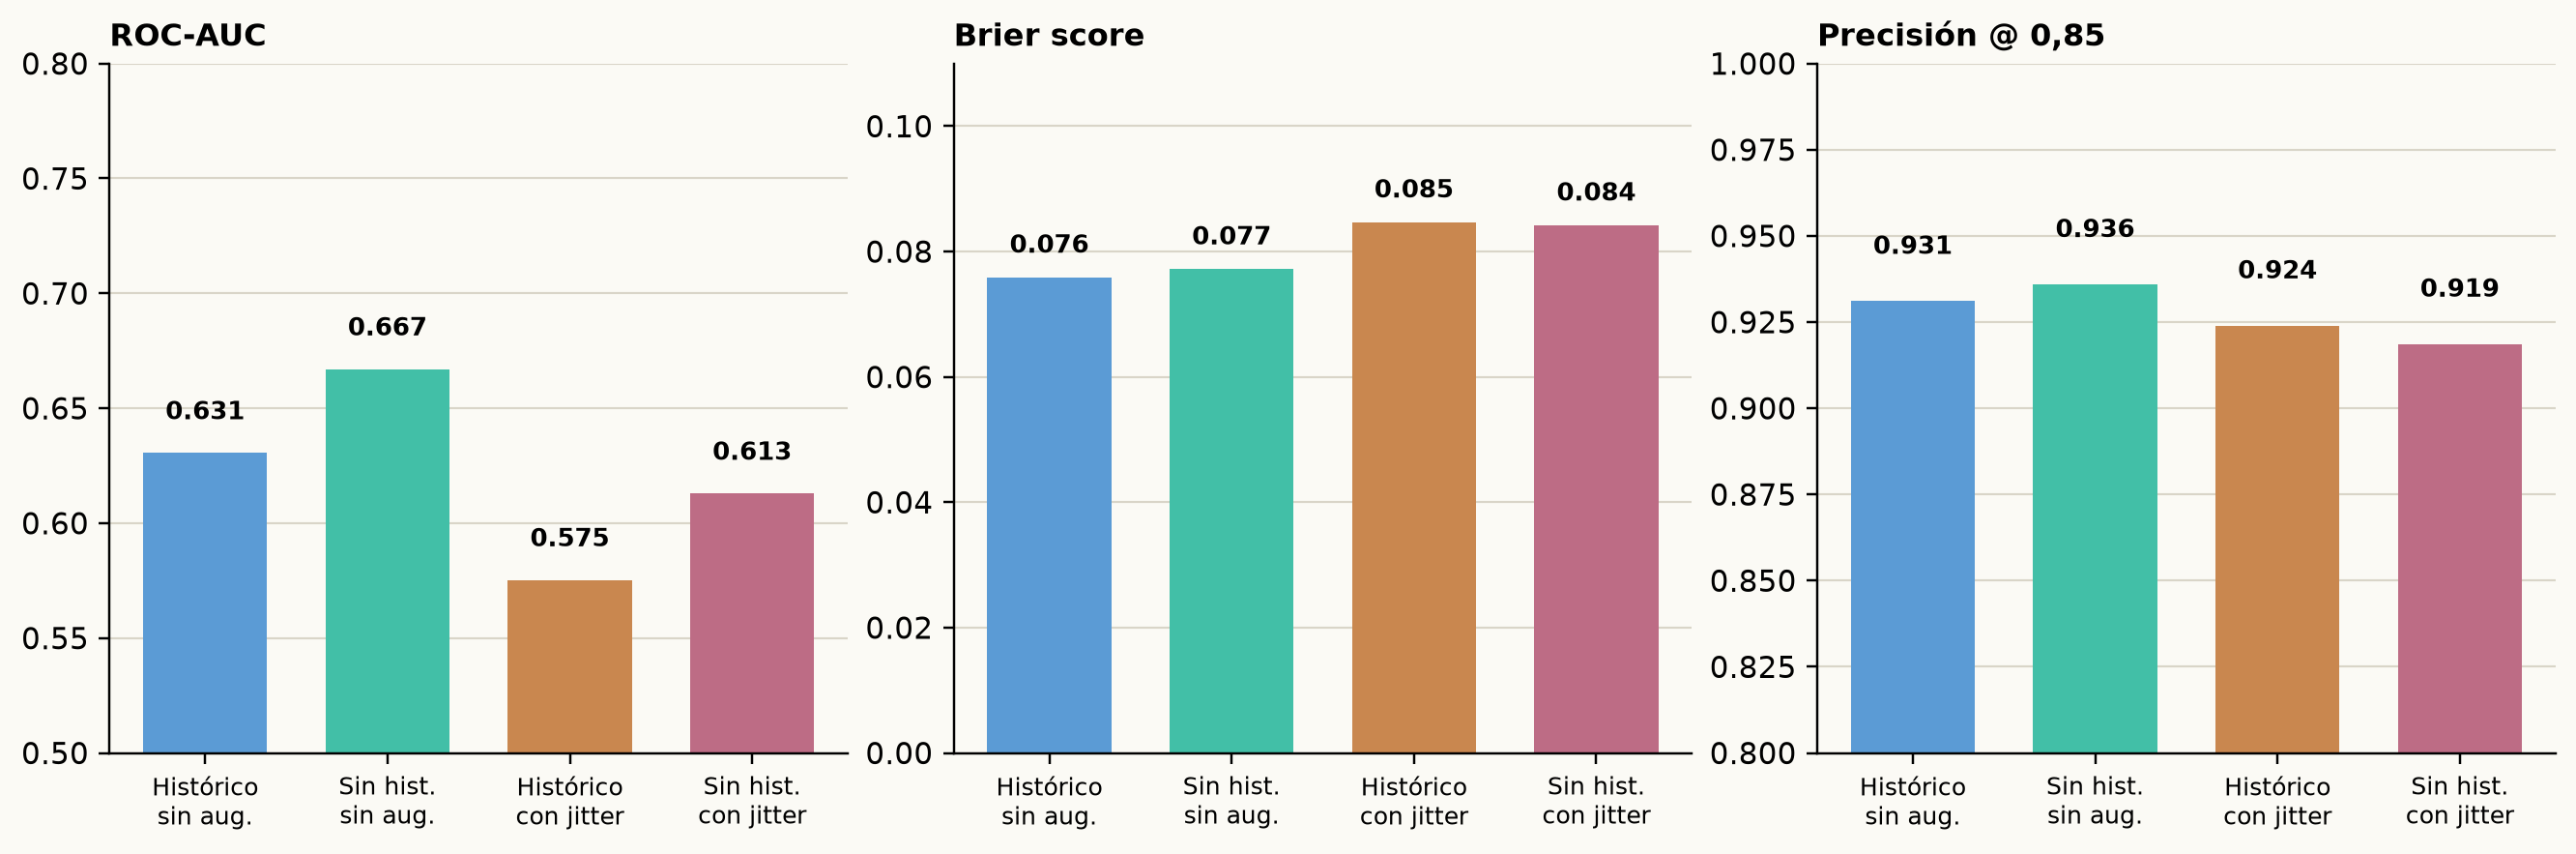
\includegraphics[width=\textwidth]{figures/experimentacion/02_ablacion_marzo.png}
\caption{Histórico y aumentación.}
\label{fig:ablacion-marzo}
\end{figure}

La combinación sin variables históricas ni perturbación numérica obtiene el mejor equilibrio entre separación y calibración. La perturbación duplica el tamaño de entrenamiento de 171 a 342 filas, pero empeora ROC-AUC y \emph{Brier} en ambas configuraciones. Por ello no se incorpora al modelo de referencia. Este resultado no prueba que la aumentación sea perjudicial en cualquier muestra. Indica que, con una colección corta y muy concentrada en operaciones positivas, introducir pequeñas variaciones de precio añade más ruido que información.

La lectura debe mantenerse prudente. Los 19 artículos disponibles en el corte aparecen tanto en entrenamiento como en prueba y la etiqueta positiva representa el 89,5\% de la prueba. Una estrategia que marca muchos casos como favorables puede alcanzar precisión elevada por la propia distribución de la muestra. El corte de mayo confirma este problema: de 361 ejemplos de entrenamiento, 76 de validación y 95 de prueba, las dos últimas particiones contienen exclusivamente etiquetas positivas. En esas condiciones ROC-AUC no es una métrica definida y no se entrena un modelo para presentarlo como comparación válida. Este resultado establece una condición de continuación clara: ampliar la cobertura cruzada BUFF--Steam y equilibrar los eventos antes de convertir el modelo en recomendación operativa.

\begin{figure}[htbp]
\centering
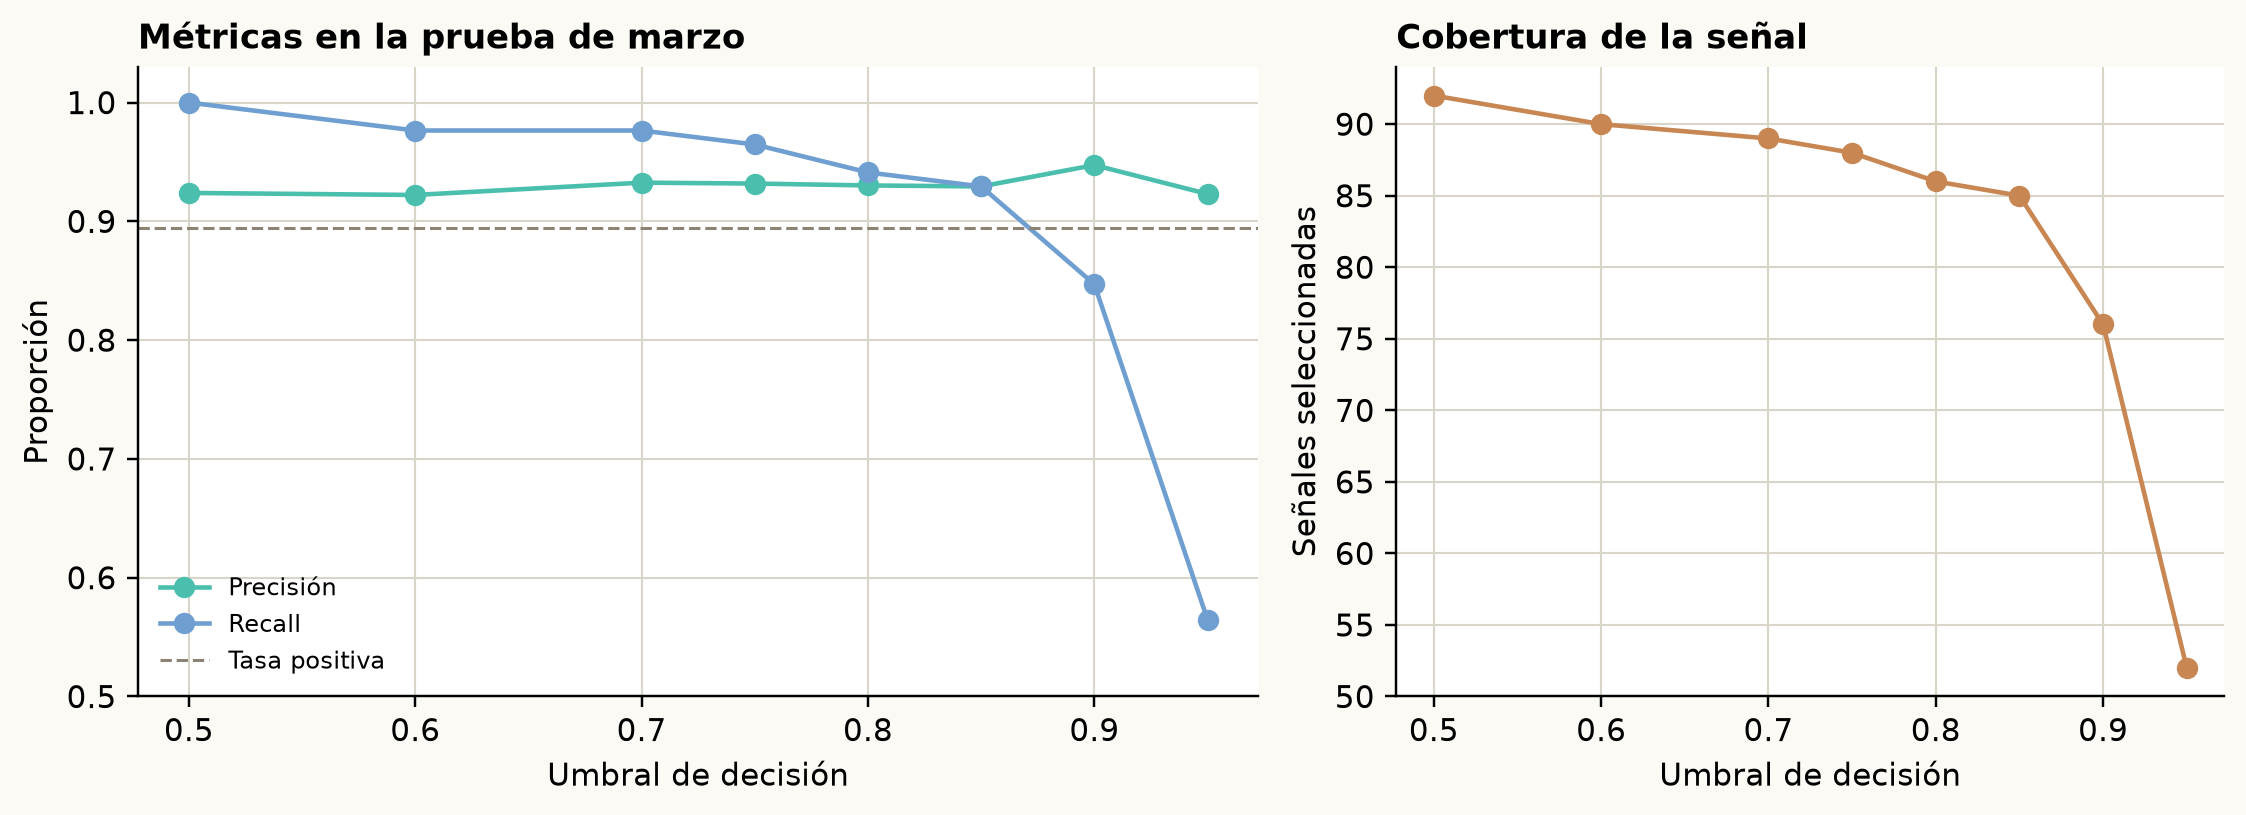
\includegraphics[width=\textwidth]{figures/experimentacion/04_umbral_marzo.png}
\caption{Métricas por umbral.}
\label{fig:umbral-marzo}
\end{figure}

La Figura~\ref{fig:umbral-marzo} complementa esta lectura. La precisión se mantiene cerca de la tasa positiva de la prueba mientras el umbral aumenta, pero el número de señales solo cae de forma apreciable a partir de 0,90. Por tanto, un umbral alto no convierte por sí mismo la señal en evidencia de selección robusta. La calibración y la precisión deben volver a evaluarse cuando haya una proporción relevante de operaciones no rentables.

\subsection{Aprendizaje MARL}

\textbf{Matriz de problemas MARL.} La matriz de entrenamiento no se limita a variar parámetros del algoritmo. Cada ejecución define un problema de cartera por la combinación de conjunto de activos, saldo inicial, periodo temporal y restricciones operativas. Los activos se seleccionan de forma estratificada por su precio mediano usando exclusivamente las particiones de entrenamiento y validación de \texttt{trading\_profit\_v2}; el bloque de prueba no interviene ni en esta selección ni en el entrenamiento. Los episodios recorren ventanas temporales consecutivas de catorce días de esos dos bloques.

La tipología de un problema se describe mediante dos dimensiones independientes: el tamaño del universo de activos y el perfil de restricciones de la cartera. Los tamaños se construyen con los activos seleccionados de forma estratificada y con las filas correspondientes de entrenamiento y validación:

\begin{itemize}
  \item \textbf{Pequeño:} cinco activos, 252 filas de entrenamiento y 66 de validación, con 500~EUR de saldo inicial.
  \item \textbf{Mediano:} veinte activos, 939 filas de entrenamiento y 257 de validación, con 1.000~EUR de saldo inicial.
  \item \textbf{Grande:} cien activos, 4.884 filas de entrenamiento y 1.316 de validación, con 5.000~EUR de saldo inicial.
\end{itemize}

El perfil de cartera fija cuánto se puede invertir y concentrar. Se han definido los cuatro perfiles siguientes:

\begin{itemize}
  \item \textbf{Restrictivo:} posición máxima del 10\,\%, exposición por artículo del 15\,\%, exposición por plataforma del 50\,\%, reserva mínima de efectivo del 25\,\%, objetivo de inversión del 35\,\% y como máximo tres posiciones abiertas.
  \item \textbf{Estándar:} posición máxima del 20\,\%, exposición por artículo del 30\,\%, exposición por plataforma del 70\,\%, reserva mínima del 10\,\% y objetivo de inversión del 50\,\%. El máximo de posiciones se ajusta al tamaño: ocho en el caso mediano y veinte en el grande.
  \item \textbf{Concentrado:} posición máxima del 30\,\%, exposición por artículo del 60\,\%, exposición por plataforma del 90\,\%, reserva mínima del 5\,\%, objetivo de inversión del 65\,\% y como máximo tres posiciones abiertas.
  \item \textbf{Diversificado:} posición máxima del 15\,\%, exposición por artículo del 20\,\%, exposición por plataforma del 70\,\%, reserva mínima del 10\,\%, objetivo de inversión del 65\,\% y como máximo doce posiciones abiertas.
\end{itemize}

La cuadrícula combina los tres tamaños con los cuatro perfiles: doce problemas y, con tres semillas por problema, 36 entrenamientos independientes. Para cada tamaño se conserva el mismo conjunto de activos en los cuatro perfiles, de modo que las diferencias observadas puedan atribuirse a las restricciones de cartera y no a un cambio de artículos. La matriz se ha ejecutado íntegramente sobre entrenamiento y validación; el bloque de prueba no interviene en la selección ni en estas comparaciones.

Todas las ejecuciones usan tres políticas, \textit{Scout}, \textit{Trader} y \textit{Portfolio}, con \acroref{PPO}{PPO}, tasa de aprendizaje $0{,}0003$, descuento $\gamma=0{,}99$, ocho episodios por iteración y un máximo de ochenta iteraciones. La recompensa combina un componente común, con peso $g=0{,}70$, y señales específicas de cada rol. La parada temprana se activa después de veinte iteraciones sin mejora del retorno de cartera en validación. Las políticas comienzan con salidas \emph{logit} neutras; por tanto, sin evidencia de aprendizaje no favorecen inicialmente ninguna acción válida.

\textbf{Métricas de aprendizaje.} Además del retorno de validación, se registra la recompensa común por paso, las recompensas de \textit{Scout}, \textit{Trader} y \textit{Portfolio}, la entropía de cada política, las probabilidades medias de sus acciones, la pérdida de la red \emph{actor}, la fracción de actualizaciones recortadas y la divergencia KL aproximada. Para el crítico central se registra la pérdida de valor, que es el error cuadrático medio entre el retorno estimado y el valor predicho. Estas métricas distinguen una cartera que obtiene un retorno puntual de un proceso en el que las políticas cambian de forma coherente y el crítico se mantiene estable.

\begin{figure}[H]
\centering
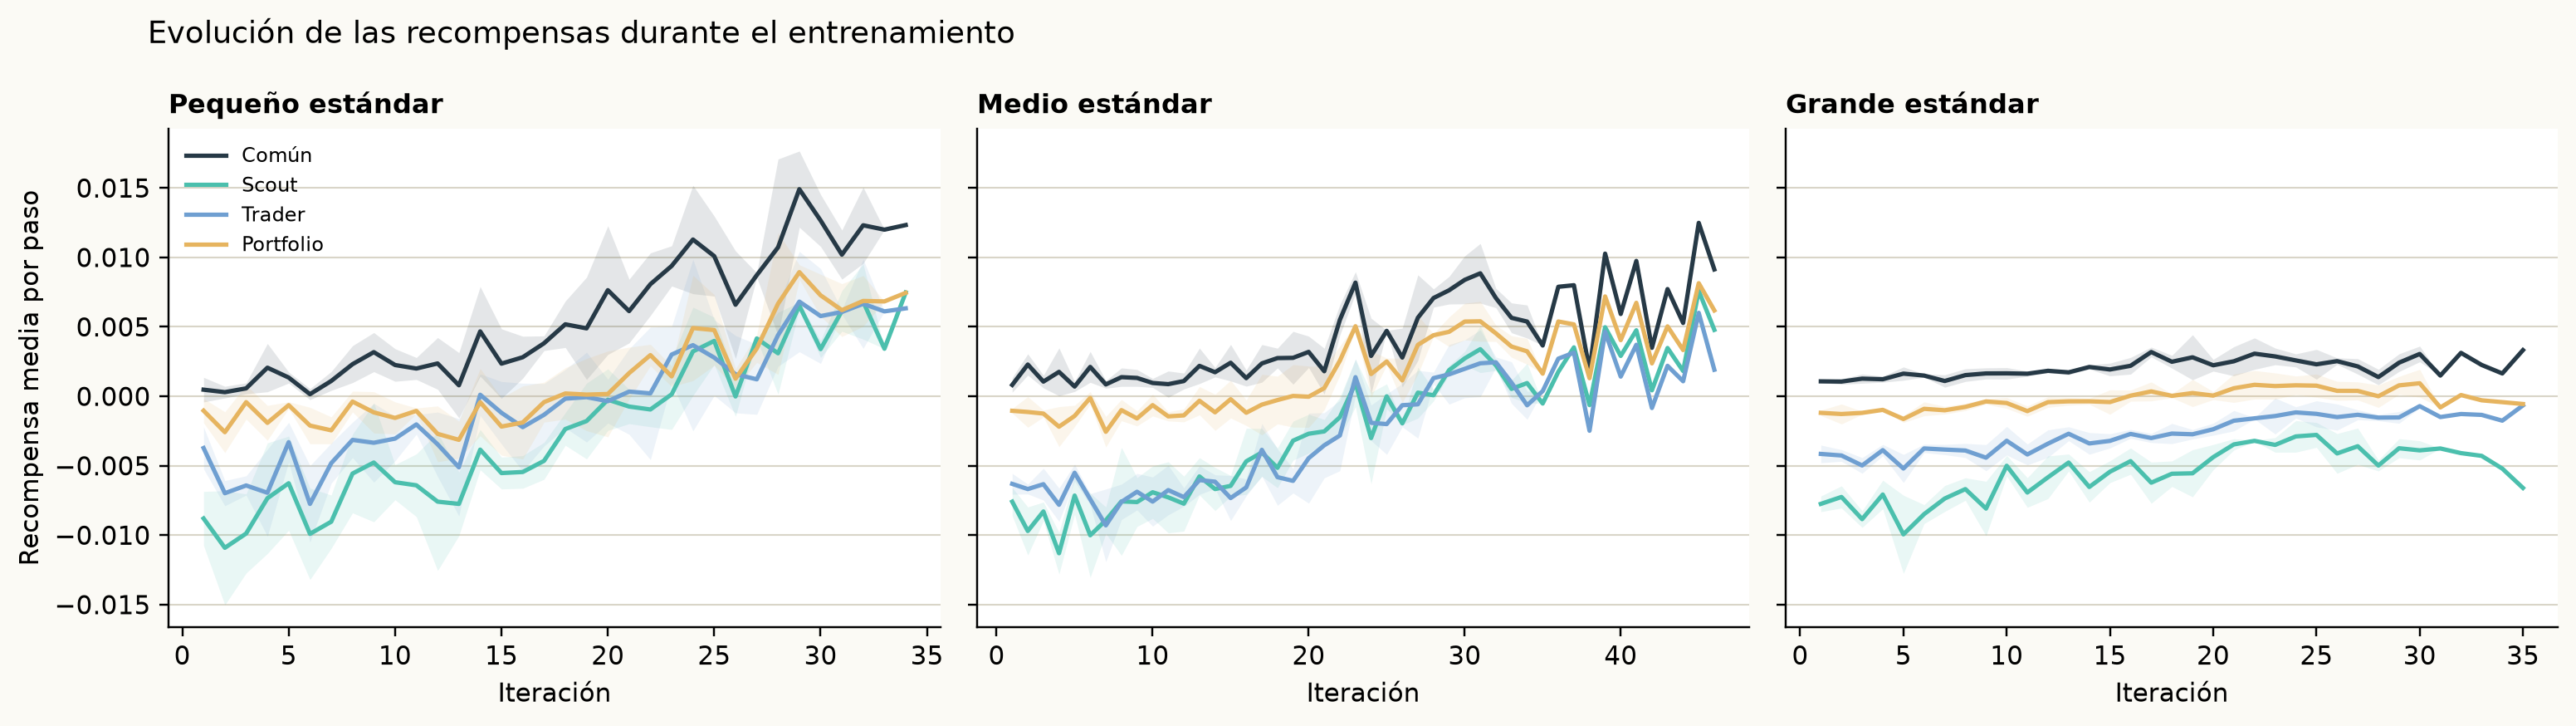
\includegraphics[width=\textwidth]{figures/experimentacion/09_marl_recompensas.png}
\caption{Recompensas durante el entrenamiento.}
\label{fig:marl-recompensas}
\end{figure}

La Figura~\ref{fig:marl-recompensas} muestra la media y la variabilidad entre semillas de los tres tamaños con perfil estándar. En los escenarios pequeño y medio, la recompensa común y las señales de los roles aumentan durante el entrenamiento. En el escenario grande, en cambio, la mejora es más tenue y la señal de \textit{Scout} permanece negativa. La comparación indica que aumentar el número de activos sin aumentar el presupuesto de entrenamiento no produce la misma evidencia de aprendizaje.

\begin{figure}[H]
\centering
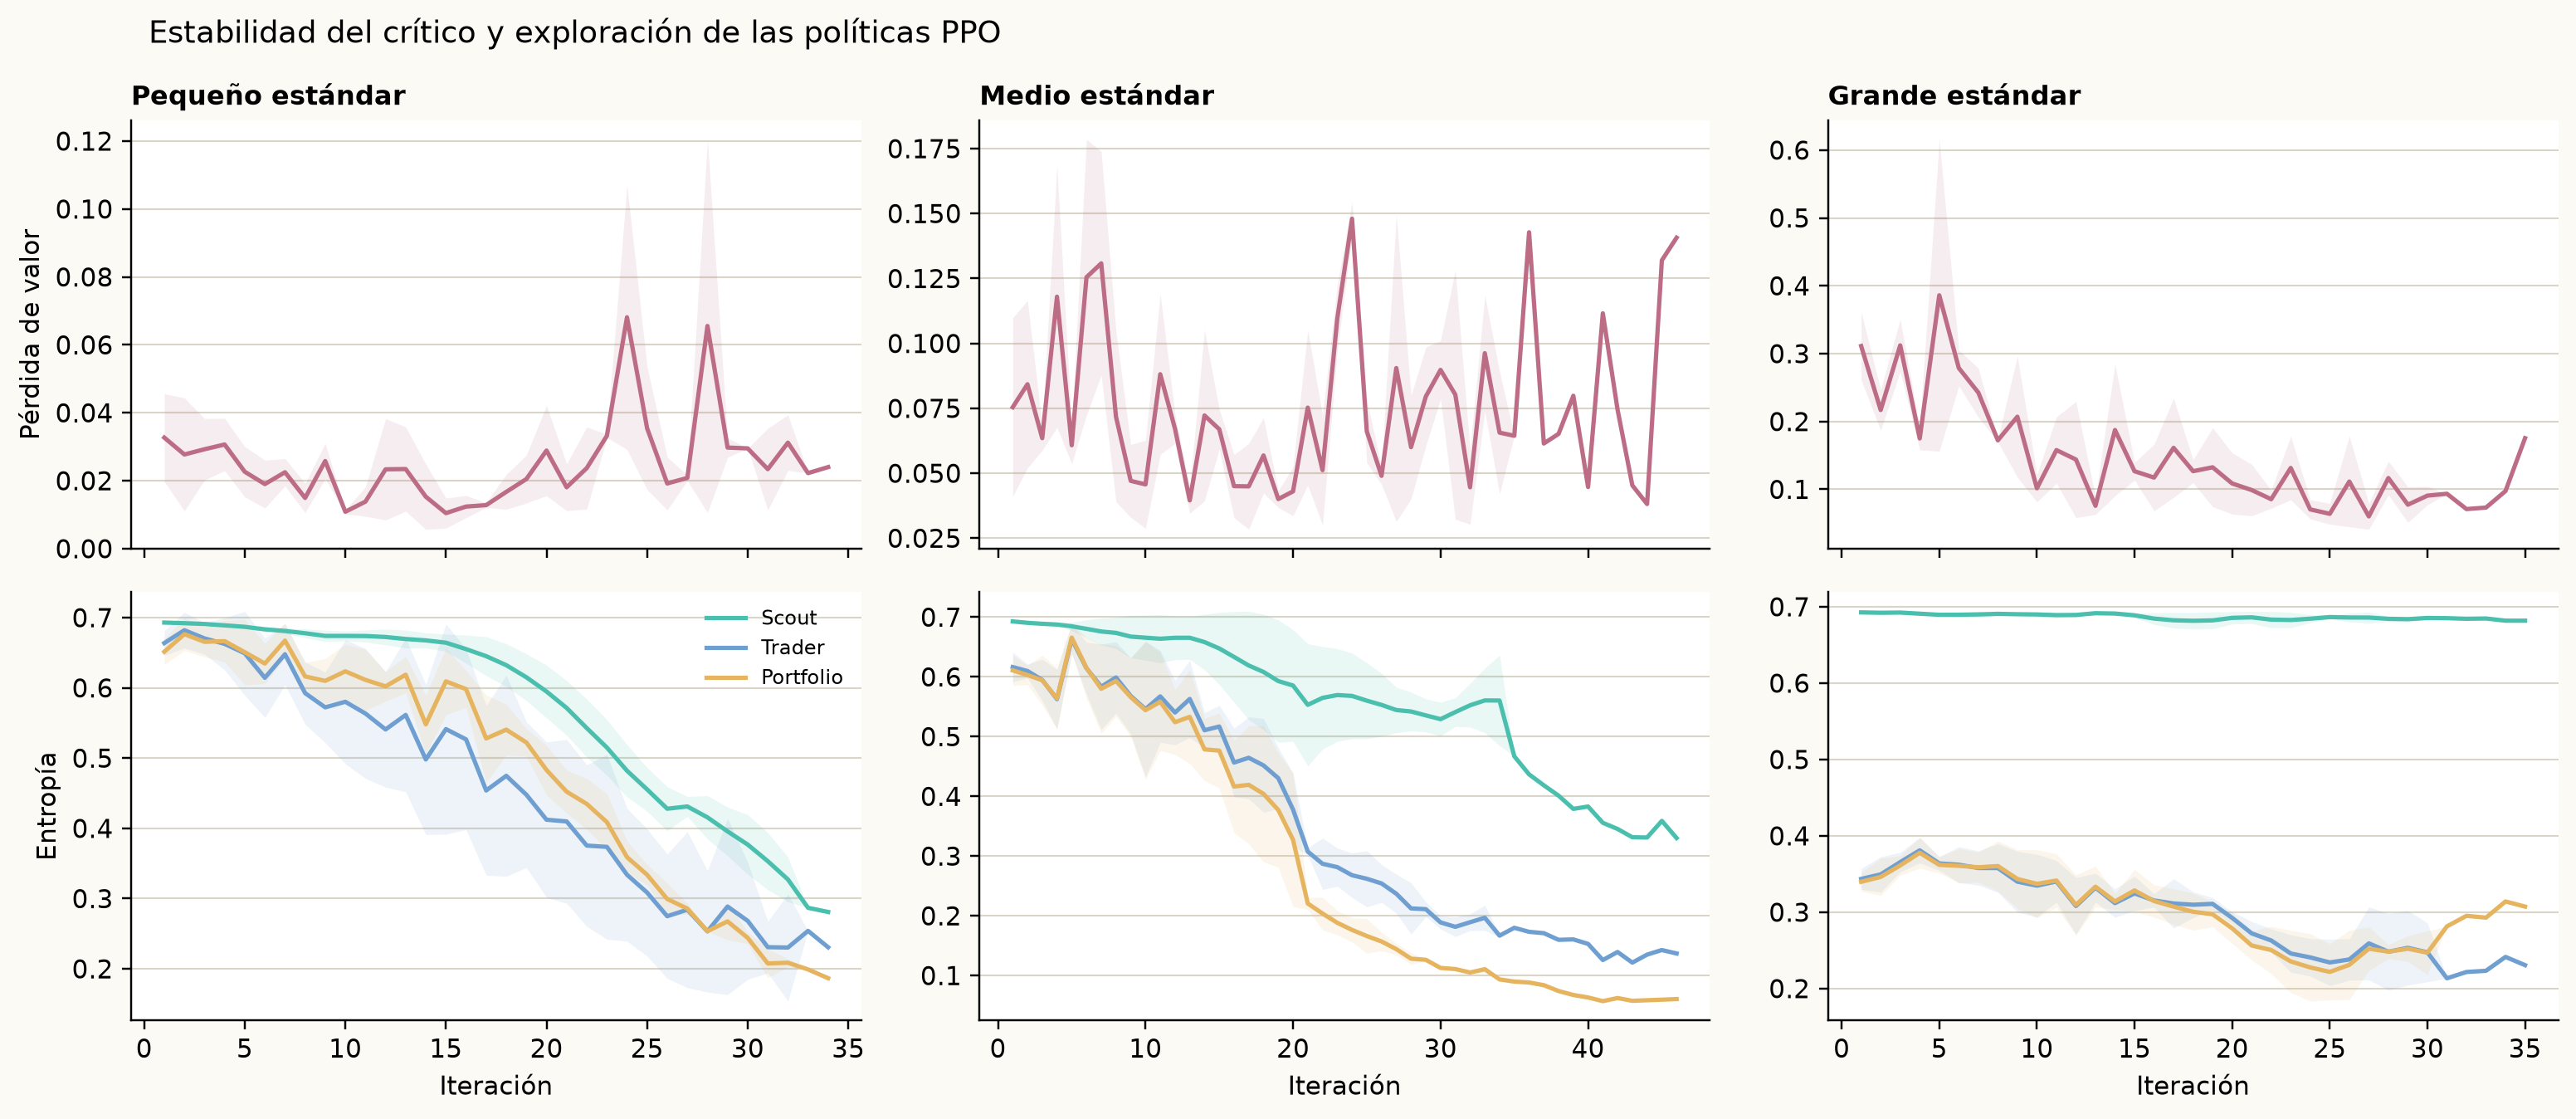
\includegraphics[width=\textwidth]{figures/experimentacion/10_marl_estabilidad_ppo.png}
\caption{Estabilidad del entrenamiento con PPO.}
\label{fig:marl-estabilidad}
\end{figure}

La Figura~\ref{fig:marl-estabilidad} completa el diagnóstico. La pérdida de valor del crítico disminuye de forma global en los tres casos, aunque mantiene oscilaciones propias de las actualizaciones por lotes. Las entropías bajan con claridad para \textit{Trader} y \textit{Portfolio} en los escenarios pequeño y medio: las políticas dejan de explorar sus acciones con probabilidades similares. En el escenario grande, la entropía de \textit{Scout} casi no cambia, otra señal de que el entrenamiento disponible resulta insuficiente para esa escala.

\begin{figure}[H]
\centering
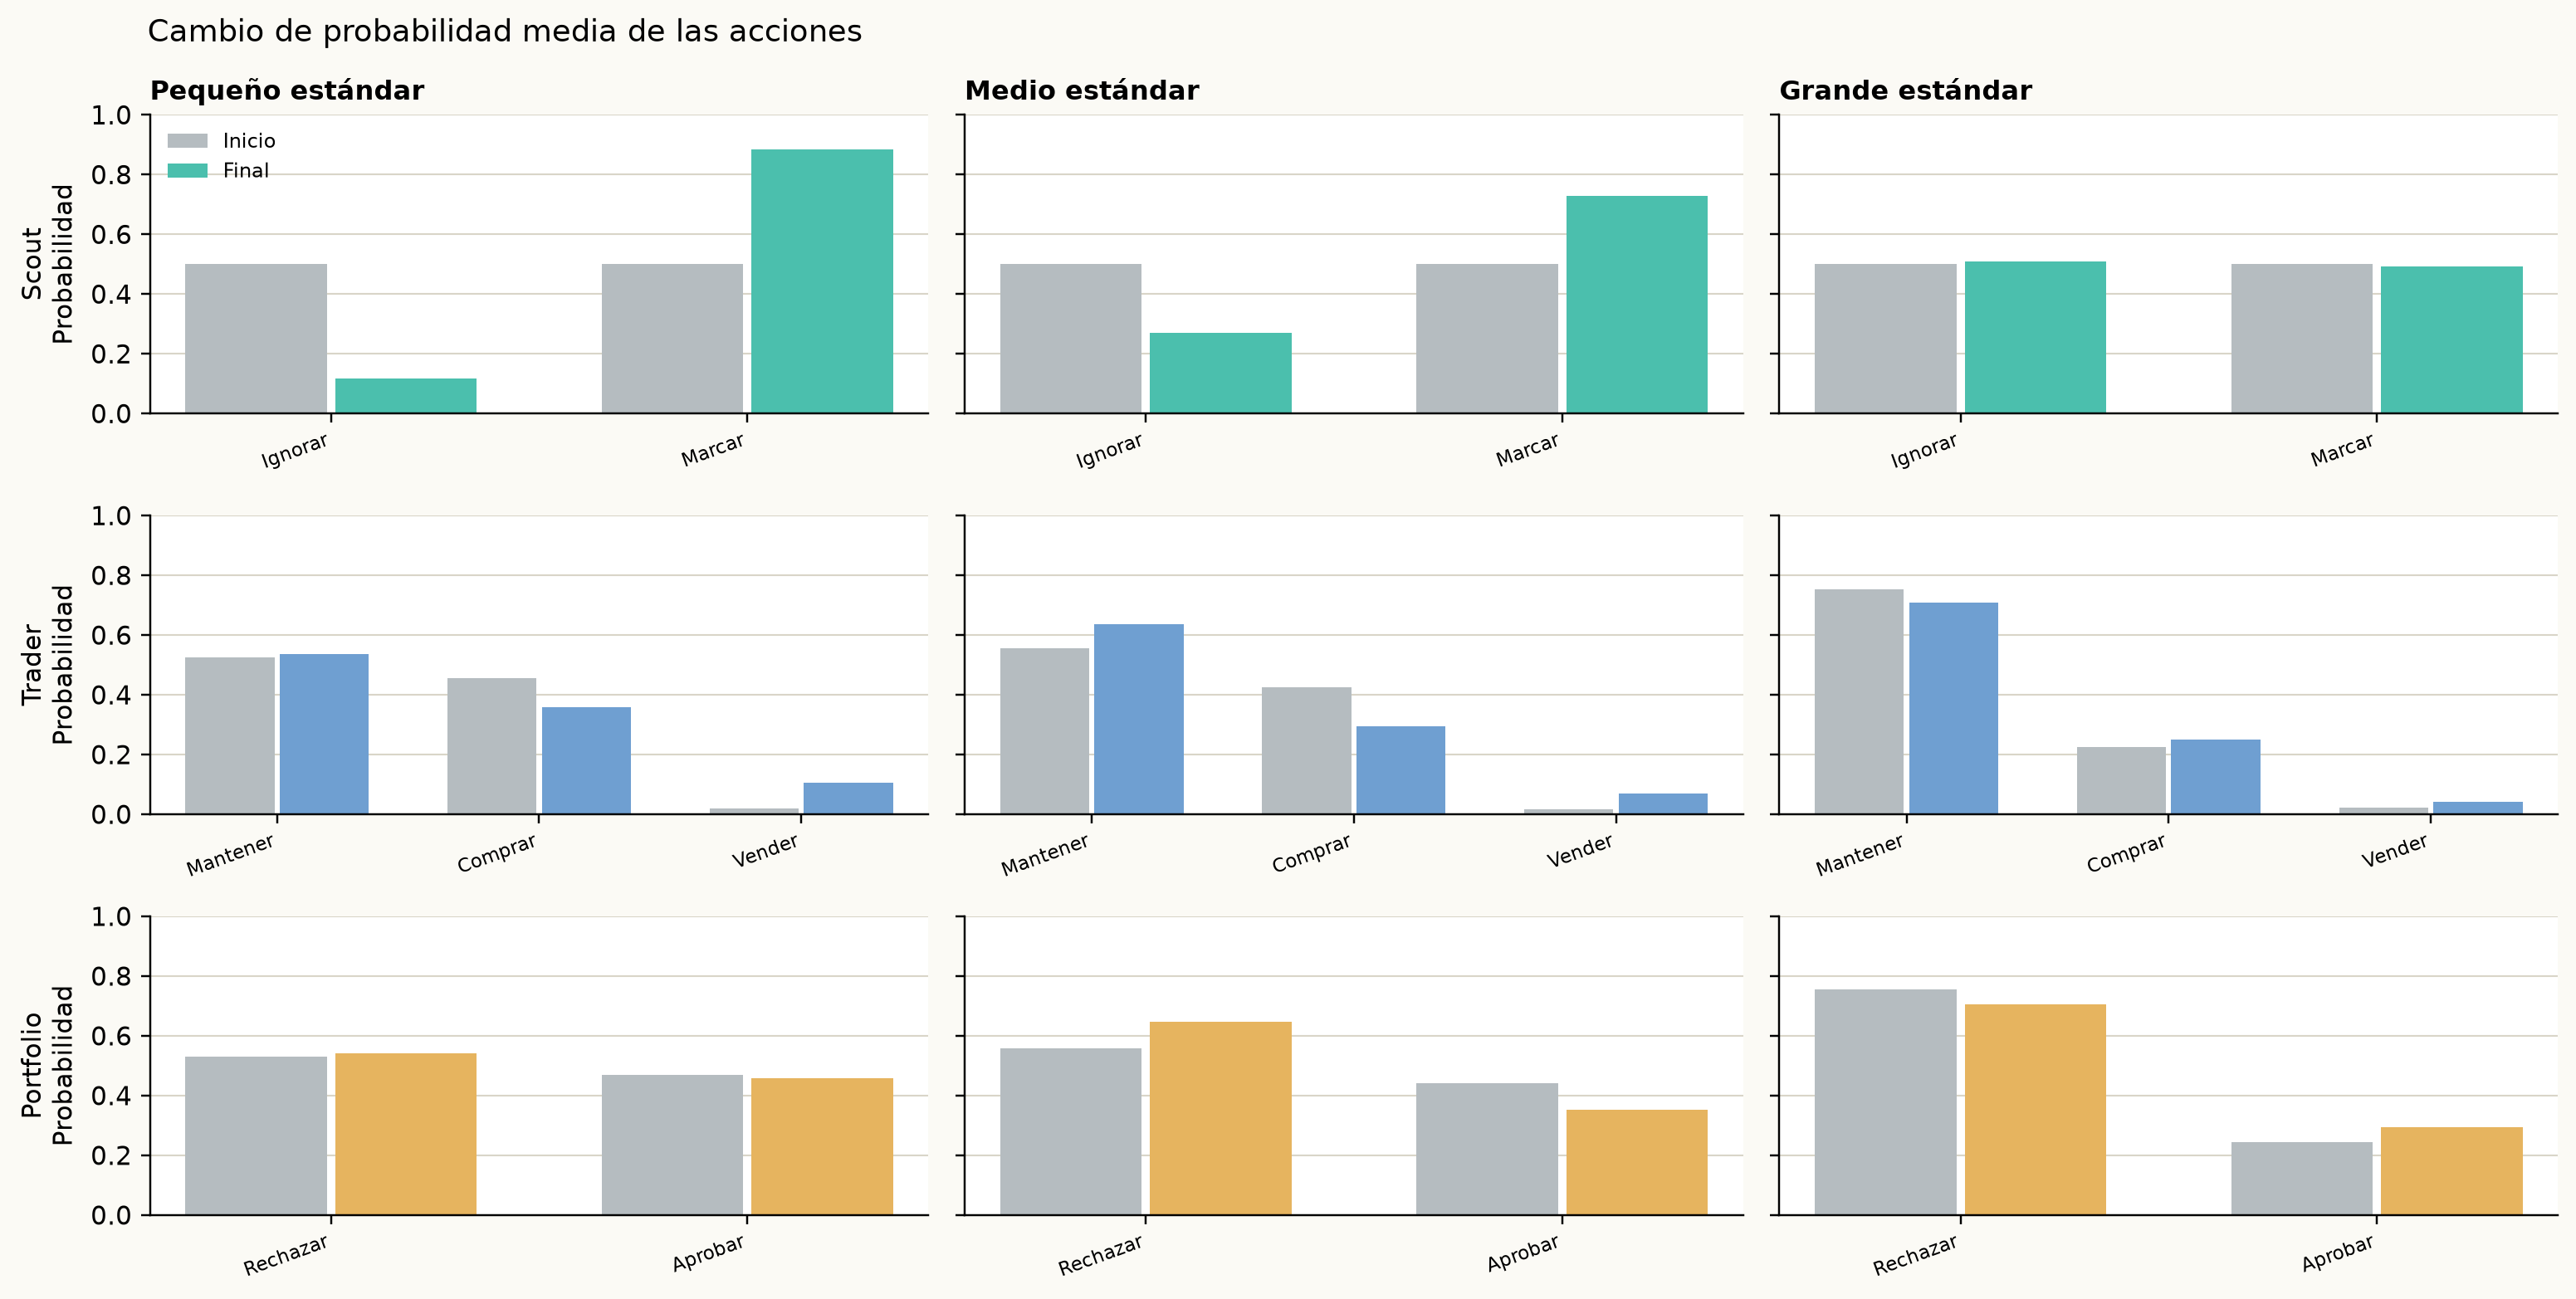
\includegraphics[width=\textwidth]{figures/experimentacion/11_marl_politicas.png}
\caption{Políticas al inicio y al final del entrenamiento.}
\label{fig:marl-politicas}
\end{figure}

La modificación de las políticas puede verse de forma directa en la Figura~\ref{fig:marl-politicas}. \textit{Scout} pasa de repartir su probabilidad entre ignorar y marcar a priorizar marcar en los problemas pequeño y medio; \textit{Trader} aumenta la probabilidad de mantener y reduce la de comprar; y \textit{Portfolio} modifica el equilibrio entre aprobar y rechazar. El escenario grande conserva probabilidades próximas a las iniciales. Esta evidencia no prueba que las decisiones sean óptimas, pero sí muestra qué agentes han abandonado la política inicial neutra y hacia qué acciones se han desplazado.

\section{Resultados económicos}

Esta sección mide el valor de una única cartera conjunta. Primero se emplea validación para seleccionar una tipología; después se compara esa selección una sola vez sobre la prueba aislada. Los retornos de validación sirven para elegir una configuración y no deben interpretarse como una estimación independiente de rentabilidad.

\subsection{Selección económica en validación}

La Tabla~\ref{tab:resultados-tipologias-marl} resume el retorno de cartera de las doce combinaciones durante la validación. El retorno es el aumento del valor final de cartera respecto al saldo inicial en el mejor punto de control de cada semilla. El perfil diversificado obtiene el mayor retorno medio en los tres tamaños; la combinación mediano-diversificada alcanza 3,504\,\%, aunque su intervalo de 0,000 a 5,255\,\% muestra que una semilla no mejora el retorno inicial. Por tanto, el resultado identifica una tipología para la prueba, no una configuración superior de forma concluyente.

\begin{table}[htbp]
\centering
\begin{tabularx}{\textwidth}{>{\raggedright\arraybackslash}X >{\raggedright\arraybackslash}l r r}
\toprule
Tamaño & Perfil & Retorno medio & Intervalo entre semillas \\
\midrule
Pequeño & Restrictivo & 0,377\,\% & 0,377--0,377\,\% \\
Pequeño & Estándar & 0,609\,\% & 0,383--1,061\,\% \\
Pequeño & Concentrado & 0,377\,\% & 0,377--0,377\,\% \\
Pequeño & Diversificado & 0,896\,\% & 0,880--0,904\,\% \\
Mediano & Restrictivo & 1,161\,\% & 0,719--1,382\,\% \\
Mediano & Estándar & 1,976\,\% & 0,000--3,123\,\% \\
Mediano & Concentrado & 1,261\,\% & 1,201--1,382\,\% \\
Mediano & Diversificado & \textbf{3,504\,\%} & 0,000--5,255\,\% \\
Grande & Restrictivo & 0,260\,\% & 0,190--0,401\,\% \\
Grande & Estándar & 1,707\,\% & 1,623--1,816\,\% \\
Grande & Concentrado & 0,250\,\% & 0,190--0,370\,\% \\
Grande & Diversificado & 1,878\,\% & 1,623--2,006\,\% \\
\bottomrule
\end{tabularx}
\caption{Validación MARL por escenario.}
\label{tab:resultados-tipologias-marl}
\end{table}

\begin{figure}[H]
\centering
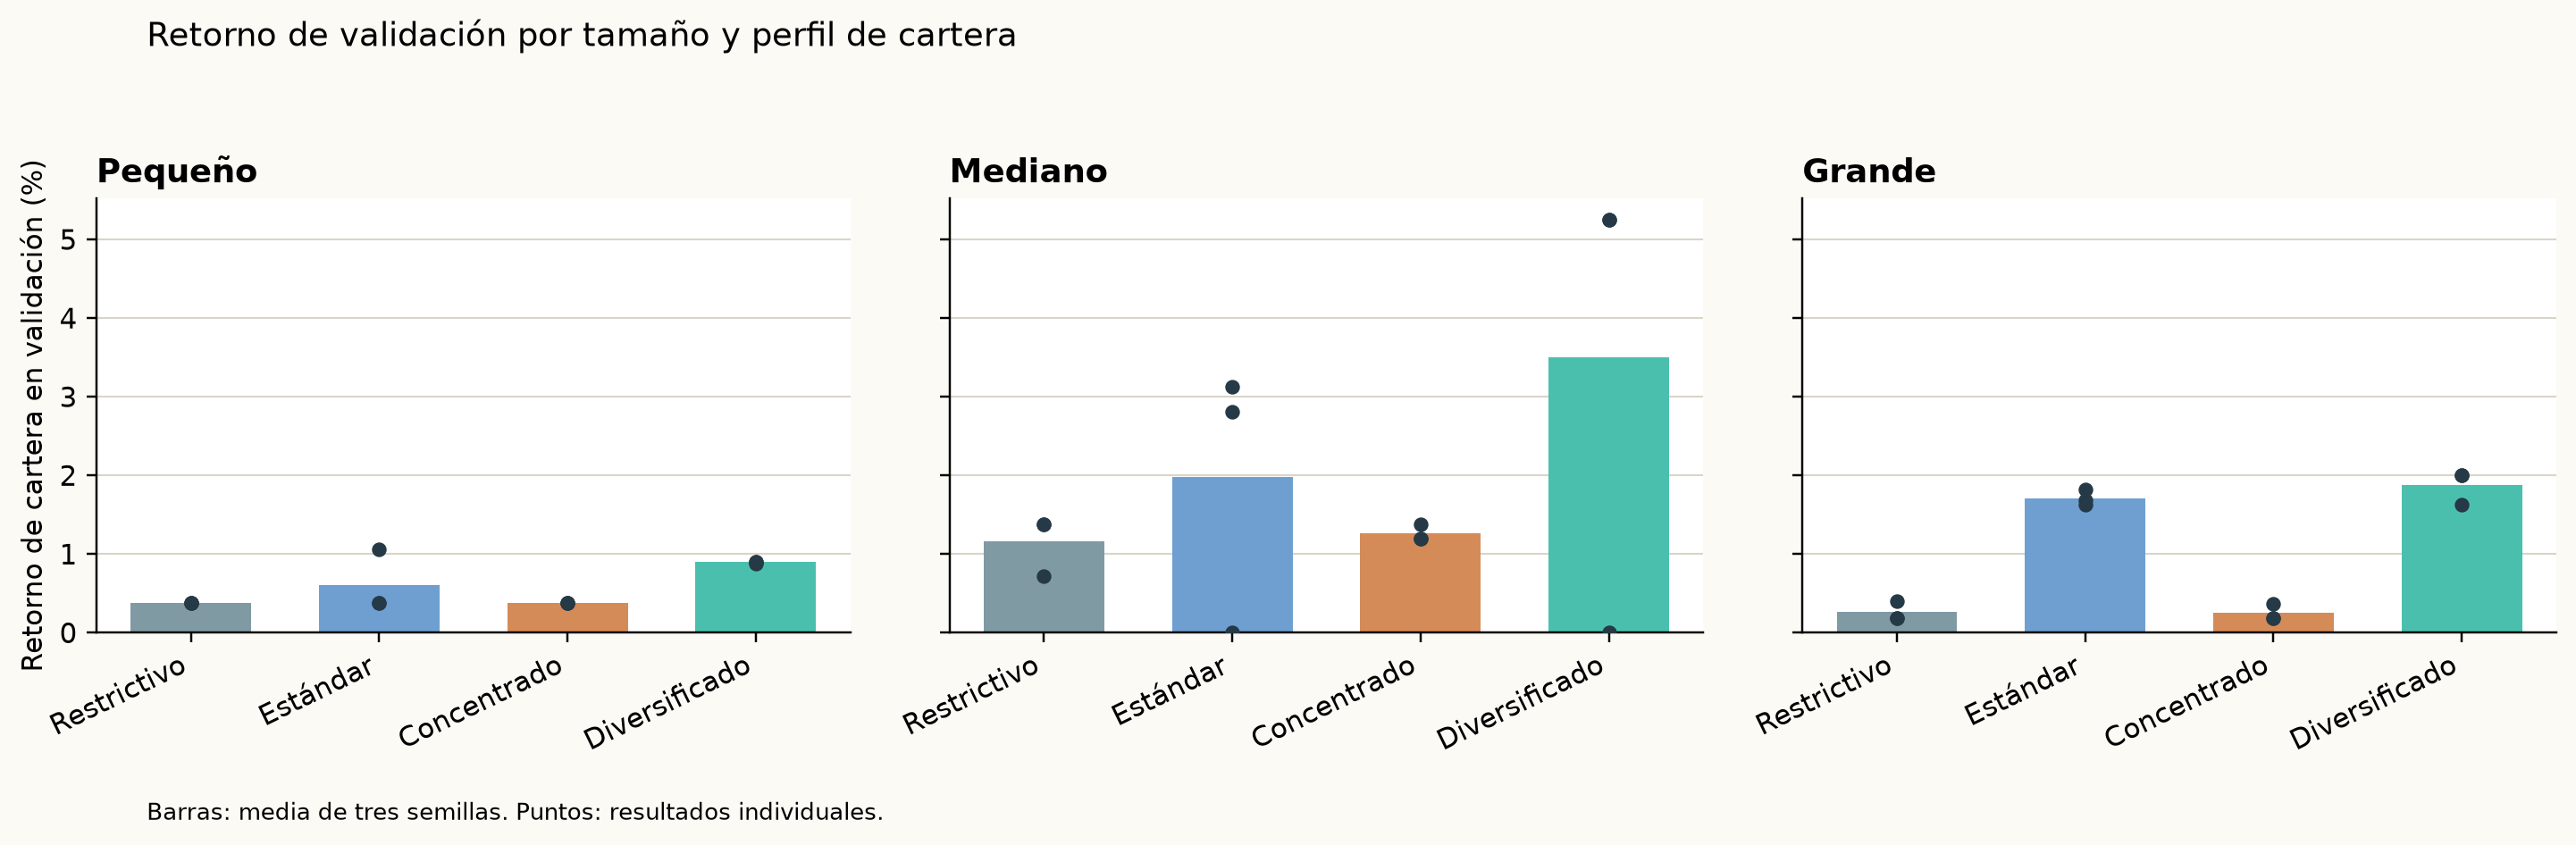
\includegraphics[width=\textwidth]{figures/experimentacion/12_marl_cuadricula_completa.png}
\caption{Retorno de validación por escenario.}
\label{fig:marl-cuadricula-completa}
\end{figure}

La Figura~\ref{fig:marl-cuadricula-completa} permite comparar los perfiles dentro de un mismo tamaño. La diversificación mejora el retorno medio frente a los perfiles restrictivo y concentrado en los tres tamaños. No obstante, la dispersión observada en el caso mediano aconseja no usar solo la media para seleccionar una política. Las curvas de recompensa, entropía y pérdida de valor mostradas anteriormente complementan este resultado: el escenario grande mantiene mayor entropía de \textit{Scout}, mientras que el mediano diversificado alcanza retornos más altos a costa de una variabilidad notable entre semillas.

\subsection{Evaluación independiente en prueba}

Una vez elegida la tipología media diversificada mediante validación, se ha realizado una única evaluación sobre el bloque de prueba. Los tres checkpoints MARL, las tres réplicas de la referencia PPO centralizada formada por una única política, la regla de margen neto positivo y la política de mantener efectivo recorren las mismas ocho ventanas temporales, con los mismos veinte activos, 1.000~EUR y restricciones. La política centralizada observa el estado global y escoge la acción conjunta, mientras que los tres roles MARL actúan con sus observaciones locales. En todas las filas se mide el valor de una única cartera conjunta, no el rendimiento aislado de cada rol.

La Tabla~\ref{tab:prueba-final-marl} muestra el resultado económico y el uso de efectivo. MARL obtiene un retorno medio de 6,605\,\%, con un intervalo entre semillas de 6,163--6,869\,\%, y 66,05~EUR de beneficio realizado; supera a mantener efectivo y a la política PPO centralizada, cuyo promedio queda condicionado por una semilla que no mejora en validación. Sin embargo, la regla determinista de margen positivo alcanza 7,098\,\%. La diferencia de 0,493 puntos porcentuales no permite presentar la arquitectura multiagente como superior a esa referencia simple.

\begin{table}[htbp]
\centering
\small
\begin{tabularx}{\textwidth}{>{\raggedright\arraybackslash}X r r r r}
\toprule
Política & Retorno medio & Beneficio neto & Efectivo final & Capital bloqueado \\
\midrule
Mantener efectivo & 0,000\,\% & 0,00~EUR & 1.000,00~EUR & 0,00~EUR \\
Margen neto positivo & \textbf{7,098\,\%} & \textbf{70,98~EUR} & 716,06~EUR & 326,34~EUR \\
PPO centralizado & 4,486\,\% & 44,86~EUR & 815,60~EUR & 210,21~EUR \\
MARL (tres roles) & 6,605\,\% & 66,05~EUR & 685,63~EUR & 336,75~EUR \\
\bottomrule
\end{tabularx}
\caption{Resultado económico y capital inmovilizado en prueba.}
\label{tab:prueba-final-marl}
\end{table}

La Tabla~\ref{tab:riesgo-prueba-final} completa la comparación con la actividad de cartera y las restricciones. MARL cierra una media de 11 operaciones y conserva 12 posiciones abiertas, por lo que una parte relevante de su valor final permanece inmovilizada. La política de margen positivo presenta un uso de capital muy parecido. PPO centralizado bloquea menos capital, pero también obtiene menor retorno y su media incluye una réplica que no opera.

\begin{table}[htbp]
\centering
\begin{tabularx}{\textwidth}{>{\raggedright\arraybackslash}X r r r r}
\toprule
Política & Ventas cerradas & Posiciones abiertas & Rechazos & \emph{Drawdown} \\
\midrule
Mantener efectivo & 0,00 & 0,00 & 0,00 & 0,0000\,\% \\
Margen neto positivo & 11,25 & 12,00 & 60,00 & 0,0000\,\% \\
PPO centralizado & 7,50 & 8,00 & 40,13 & 0,0014\,\% \\
MARL (tres roles) & 11,00 & 12,00 & 59,96 & 0,0000\,\% \\
\bottomrule
\end{tabularx}
\caption{Actividad y riesgo de cartera en prueba.}
\label{tab:riesgo-prueba-final}
\end{table}

El \emph{drawdown} no discrimina las políticas en esta prueba: es nulo para MARL y para la regla de margen positivo, y prácticamente nulo para PPO centralizado. No debe interpretarse como ausencia de riesgo. El simulador valora las compras y ventas con precios históricos observados y, en estas ventanas, las posiciones cerradas no generan caídas relevantes del valor de cartera. Por ello el capital bloqueado y los rechazos informan mejor sobre la presión de las restricciones en el experimento actual; para evaluar caídas de cartera de forma realista se necesitarían trayectorias con pérdidas y precios de liquidación no conocidos de antemano.

\section{Discusión}

Esta sección interpreta los resultados obtenidos, sin añadir experimentos nuevos. Su objetivo es delimitar qué evidencia aporta el trabajo, qué condiciones reducen la solidez de las conclusiones y qué falta para comparar una política multiagente con una estrategia simple.

\subsection{Evolución del enfoque experimental}

La construcción y calidad de los conjuntos descritas en la Sección~\ref{sec:calidad-conjunto-experimental} han condicionado el alcance de cada experimento. El primer conjunto de compraventa permitió verificar el cálculo de etiquetas y costes, pero no sirvió para medir un modelo por su falta de clases en validación y prueba. Las correcciones en la lectura de datos, la normalización de moneda y la recuperación de histórico condujeron al conjunto \texttt{trading\_profit\_v2}, que ya contiene operaciones rentables y no rentables en las tres particiones temporales. Aun así, la proporción de operaciones rentables sigue siendo elevada, por lo que sus resultados no equivalen a una garantía de rentabilidad futura.

Esta evolución también ha permitido separar dos objetivos que no deben confundirse. La ruta BUFF--Steam se utiliza para construir y evaluar ejemplos de compraventa con precios, comisiones y horizonte temporal definidos. En una consulta operativa, un precio de \acroref{BUFF}{BUFF} puede utilizarse como entrada actual para comprobar si conserva margen frente a una salida Steam estimada. Esta segunda aplicación no pretende predecir el precio exacto de \acroref{BUFF}{BUFF}, sino decidir si la información disponible justifica revisar una oportunidad concreta.

Por último, antes de ampliar el número de episodios y configuraciones multiagente, se priorizó que el entorno, las recompensas, las restricciones y las métricas fueran comprobables. Esta secuencia desplazó el trabajo desde reglas manuales dispersas hacia una simulación reproducible y permite interpretar la matriz de entrenamiento junto con sus límites de datos, en lugar de presentar una política como concluyente sin evidencia suficiente.

\subsection{Alcance de la evidencia y limitaciones}

La principal limitación de los resultados supervisados es el desequilibrio de etiquetas. La prueba de marzo contiene 85 operaciones rentables de 95 y los bloques posteriores llegan a tener una sola clase. Además, los mismos artículos aparecen en entrenamiento y prueba. La división por fecha evita utilizar información futura, pero no demuestra que el modelo pueda generalizar a artículos virtuales que no haya observado durante el entrenamiento. Estas condiciones hacen que una precisión elevada o una probabilidad bien calibrada deban interpretarse con cautela.

También existe una limitación operativa. El precio de \acroref{BUFF}{BUFF} se consulta como entrada puntual, mientras que la salida en Steam se estima con histórico y comisiones. Para reproducir de forma más fiel una operación entre ambas plataformas se necesitan más capturas sincronizadas y una cobertura mayor de artículos. Además, los experimentos simulan operaciones con datos observados: no envían órdenes reales, no transfieren artículos entre plataformas ni utilizan capital real. Por tanto, no permiten garantizar que una operación pueda ejecutarse en el futuro al precio previsto.

Por último, la evidencia técnica tiene alcances distintos. El \acroref{OCR}{OCR} está validado a nivel funcional, pero no dispone aún de un corpus de imágenes etiquetado con el que medir su exactitud. El entorno \acroref{MARL}{MARL} ya incluye compra, bloqueo, venta y 36 entrenamientos sobre las doce combinaciones de tamaño y perfil. Las curvas muestran aprendizaje en parte de los escenarios, pero el tamaño grande mantiene una exploración elevada de \textit{Scout} y los perfiles mediano estándar y diversificado presentan variabilidad entre semillas. La combinación mediano-diversificada se ha contrastado una vez en prueba independiente, con retorno positivo, aunque sin superar la referencia de margen neto positivo. Estas limitaciones no invalidan la arquitectura, pero acotan las conclusiones a viabilidad técnica y evidencia experimental inicial.

\textbf{Evidencia actual.}

En conjunto, el trabajo demuestra que el sistema puede integrar fuentes de datos, construir conjuntos temporales, entrenar y calibrar modelos supervisados, aplicar reglas económicas y recorrer episodios de compra, bloqueo y venta dentro de una cartera simulada. También demuestra que las políticas multiagente modifican sus recompensas, entropías y distribuciones de acción de forma medible en los escenarios pequeño y medio, y que estos cambios dependen de la escala y las restricciones de cartera. La separación entre adquisición, predicción, simulación y decisión permite comprobar cada componente y localizar un problema sin rehacer el resto del sistema.

La evidencia disponible respalda, por tanto, la viabilidad técnica de la propuesta, pero no una superioridad económica de la arquitectura multiagente. Para afirmar que una política mejora una estrategia simple será necesario ampliar la cobertura temporal, reservar nuevos bloques de prueba y repetir la comparación homogénea sin reutilizar el bloque de prueba ya evaluado.
